%!TEX root = main.tex
\chapter{Feature Point}\label{chapter:feature_point}
As it was mentioned in the introduction, there are two major methods for 3D tracking: feature-based and marker-based techniques. Marker-based 3D tracking system, requires the marker and prior knowledge about the environment to estimate the pose of camera. Some times due to some restriction about the environment (e.g. outdoor environment) and tracking situation, this task is hard ot do or impossible. Hence, it is better to rely on the features that naturally are extracted from images. In this approach, more meta informations such as a model of scene, a set contains of planer parts and some information about the camera is necessary. To make this procedure independent of 3D scene models, Vincent lepetit and Pascal Fua \cite{lepetit2005monocular} introduced a method, specially for augmented reality workspaces that can explored simultaneously both camera trajectory (tracking) and 3D world map of environment (mapping). \\
For the feature-based 3D Tracking, the whole literature can be organized into two big categories regarding to the properties of the scene, objects and images.
\begin{itemize}
\item Edge-Based methods investigate the areas with the highest value of gradient that represents edges. These methods try to make an accurate match between the projection of 3D edges in the real world and these gradient points. RAPID, Explicit Edge Extraction, and Direct Optimization on Gradient are some algorithms in this area. 
% http://en.wikipedia.org/wiki/Feature_detection_(computer_vision) for example.
\item The other methods investigate on the information that can be extracted directly from the pixels of image. These can be derived from optical flow, template matching, and feature points techniques.
% TODO: check the comma
\end{itemize}

\section{Feature Point Method (Corner-Based)} \label{sec:feature_point_method}
% TODO: check the first params
% TODO convert all feature point to the feature point and feature point
Despite of Edge-Based methods that need an overall view of the whole image to find the high gradient points and contours, The feature point-based methods just use of localized features and it is the difference key between these two approaches. An feature point is a intersection of two edges that represents a point in which the direction of these two edges changed. Consequently, the gradients of this point have a huge amount in both directions. This property can be used to detect the feature point easily.\\
Both edge-based and feature point-based techniques rely on the matching the features among the frames independent of other points. They also can handle the partial occlusions and matching errors problems and are invariant to change of illumination. The advantage of feature point-based methods compared to edge-based methods is that they are not affected by the background clutter. In fact feature points can be uniquely recognizable between all image pixels.\\
% For the rest of this master thesis, instead of feature points, we used of feature points or feature points terms.\\
After detecting the feature points of an image, we need to describe these points as a unique binary or float vectors that preserve invariance to the rotation, scale and illumination. This process in which the feature points are coded into a vector of binary or float numbers is named feature extraction. The obtained vector also is called the feature descriptor.\\

\subsection{Feature Detection} \label{subsec:feature_detection}
 The efficient detection of feature point is a crucial step for many computer vision applications. For detection of features points, attention to some properties of points should be considered as follows: \cite{forstner1986feature}
\begin{enumerate}
  \item The feature points are represented by a surrounding patch around the center.
  \item Two neighbor feature points, should be different.
  \item Two almost similar feature points (usually neighbor or from same pattern) should be ignored.
  \item The feature selection operation, should have the same result and performance in all images. It means if a point was selected as a feature point in one section of the image, it should also be selected as a feature point in the same section of the other images.
\end{enumerate}
For the first time, Harris and Stephen \cite{harris1988combined} published a new method for feature detection regarding to fact that the corner of feature point represents a variation in the gradient of the point in two directions. They used this variation for detect the feature point.\\
Currently, with the advances in the field of computer vision, many new techniques for feature detection have been developed for variety of image conditions. Some of the most versatile and popular feature detector are:
\begin{itemize}
\item SIFT \cite{lowe2004distinctive}: is the most well-known and classical approach and also the original inspiration for the other algorithms that proposed later. The advantage of SIFT is, introducing a descriptor that is invariance to scalar and rotation while it is mathematically complicated and computationally heavy. The feature points are selected based on the Difference of Gaussian (DoG). In this approach the image is expanded by a continuous function of scale known as scale space. In each scale (scale octave), the local extrema is detected by comparing the center pixel with the neighbors in space. these local extrema are SIFT feature points.

\begin{figure}[H]
\begin{tabular}{cc}
  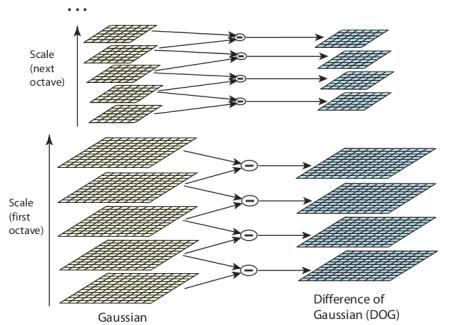
\includegraphics[width=80mm]{figures/sift_dog} &  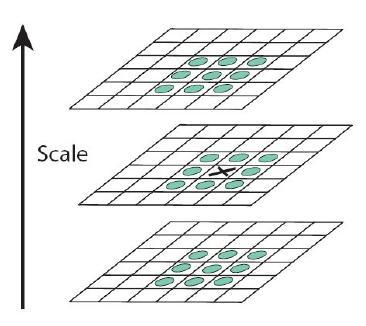
\includegraphics[width=60mm]{figures/sift_scale} \\
(a) The SIFT Difference of Gaussian (DOG) & (b) The scale octave and local extrema \\[6pt]
\end{tabular}
\caption{The SIFT feature detection processing}   \label{fig:sift_detector}
\end{figure}


\item SURF \cite{bay2006surf}: is recognized as a more efficient than the SIFT. Its detector is relied on the Hessian matrix, defined as 
\begin{equation} \label{eq:hessian_matrix}
H(x,\sigma) = \begin{bmatrix}L_{xx}(x,\sigma) & L_{xy}(x,\sigma) \\L_{xy}(x,\sigma) & L_{yy}(x,\sigma) \end{bmatrix}
\end{equation}
Where L is the convolution of the Gaussian second order derivative with the image. In implementation, the Gaussian kernel is replaced by a simple box filter. This method also is scale and rotation invariance.
 
\item FAST \cite{rosten2010faster}: is a standalone feature detector that is designed to be very efficient in real-time applications based on a light-wight complexity. A circle circle of sixteen pixels is considered around the corner candidate p.The original detector classifies p as a corner if there exists a set of n contiguous pixels in the circle which are all brighter than the intensity of the candidate pixel p plus a threshold t, or all darker than p - t. A machine learning approach is adopted and a decision tree is generated to speed up the detector. 

\begin{figure}[H]
  \centering
  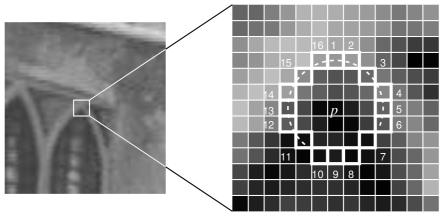
\includegraphics[width=100mm]{figures/fast_detector}
  \caption{The FAST feature detector mechanism}\label{fig:fast_detector}
\end{figure}

\item BRISK \cite{leutenegger2011brisk}: the feature point is extracted by a technique similar to the SIFT. The image is expanded into several scales (octave) and a feature point is identified at octave $i$ by analyzing the eight neighboring pixels as well as the corresponding pixels in the immediately-neighboring octaves ($i-1$ and $i+1$) above and below. In all three octaves, the local extrema is refined by a sub-pixel approach along the scale-axis to determine the true scale of the feature point.
\end{itemize}
\begin{figure}[H]
  \centering
  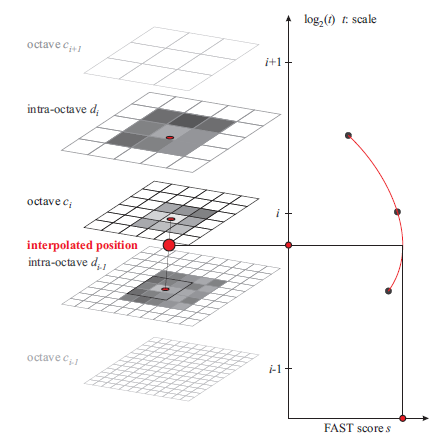
\includegraphics[width=100mm]{figures/brisk_detector}
  \caption{The BRISK feature detector}\label{fig:brisk_detector}
\end{figure}
% TODO: some methods support both feature detection and extraction but some one not

\subsection{Feature Extraction} \label{subsec:feature_extraction}
Once feature points are located, we describe a patch which surrounds the feature point as the feature descriptor. The most well-known descriptor is SIFT: A 128-dimensional float vector is obtained from a grid of histogram. This feature descriptor is created by first computing the gradient magnitude and orientation at each image sample point in a region around the feature point location (\autoref{fig:sift_descriptor}(left)). These samples are then accumulated into orientation histograms summarizing the contents over 4 x 4 subregions (\autoref{fig:sift_descriptor}(right)). The computed descriptor is robust to illumination and change of view. The other approach that its feature detector algorithm was introduced is SURF. Its idea based on local gradient histogram and it has similar performance as SIFT. The advantage of SURF algorithm over SIFT is that it is faster with less memory. Both of these approaches describe a feature point with a vector of float numbers. The SIFT uses with 128-dimensional vector and SURF with 64 or 128-dimensional vector.\\

\begin{figure}[H]
  \centering
  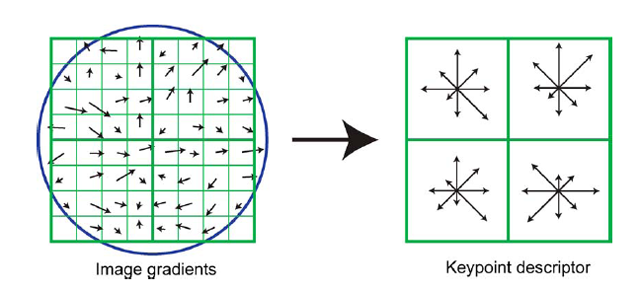
\includegraphics[width=100mm]{figures/sift_descriptor}
  \caption{The SIFT feature descriptor histogram}\label{fig:sift_descriptor}
\end{figure}

In 2010, Calonder \textit{et al.} in \cite{calonder2010brief} showed that it is possible to decrease the dimensionality of a feature descriptor by directly building a shorter binary descriptor in which all bits are pairwise independent. This new algorithm is called BRIEF. This approach is to define a test pattern (experiment indicates Gaussian distribution gives a good result) and applied to the detected feature points. The lines in (\autoref{fig:brief_descriptor}) indicates a test pair, an output of either 1 or 0 is provided based on the intensity difference of the two pixels. A series of such test outputs a binary string, which is considered as the descriptor. Representing the feature descriptor as a binary vector has the advantage of using of Hamming distance (bitwise XOR) instead of Euclidean distance for matching of the descriptors. The negative point of BRIEF algorithm however is that the result descriptor is not invariant to scale and rotation changes. After the BRIEF, both BRISK \cite{leutenegger2011brisk} and FREAK \cite{alahi2012freak} were developed that are state-of-the-art algorithms that rely on binary descriptors and are also invariant to scale and rotation. \\

\begin{figure}[H]
  \centering
  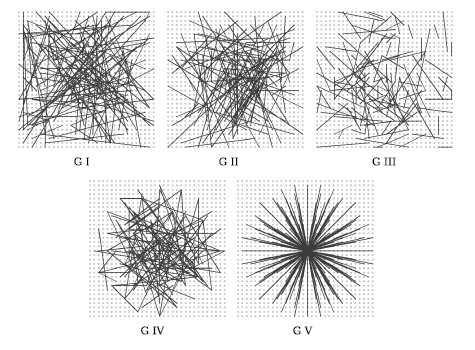
\includegraphics[width=100mm]{figures/brief_descriptor}
  \caption{The BRIEF feature descriptor}\label{fig:brief_descriptor}
\end{figure}

BRISK is a 512 bit binary descriptor that computes the weighted Gaussian average over a selected pattern of points near the feature point. The pattern is designed as that N locations are equally spaced on circles concentric with the feature point. For the formation of the rotation and scale normalized descriptor, BRISK applies the sampling pattern rotated by alpha around the feature point. The bit-vector descriptor is assembled by performing all the short-distance binary intensity comparisons of point pairs. \autoref{fig:brisk_descriptor} show the pattern of brisk.\\

\begin{figure}[H]
  \centering
  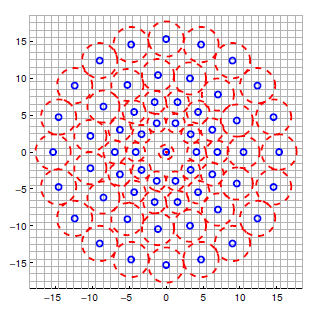
\includegraphics[width=60mm]{figures/brisk_descriptor}
  \caption{The pattern of BRISK for feature descriptor}\label{fig:brisk_descriptor}
\end{figure}

FREAK is a standalone descriptor. It improves upon the sampling pattern and method of pair selection that BRISK uses. FREAK evaluates 43 weighted Gaussians at locations around the feature point, but the pattern formed by these Gaussians is biologically inspired by the retinal pattern in the eye (\autoref{fig:freak_descriptor}(a)). The pixels being averaged overlap, and are much more concentrated near the feature point. The actual FREAK algorithm uses a cascade for comparing these pairs, and puts the 64 most important bits in front to speed up the matching process. The final pattern is shown in 
\autoref{fig:freak_descriptor}(b).

\begin{figure}[H]
\begin{tabular}{cc}
  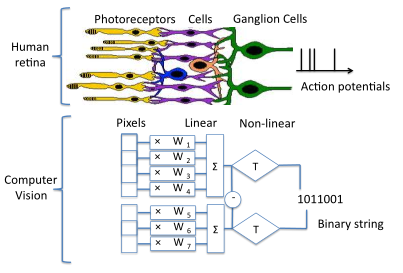
\includegraphics[width=60mm]{figures/freak_retina} &  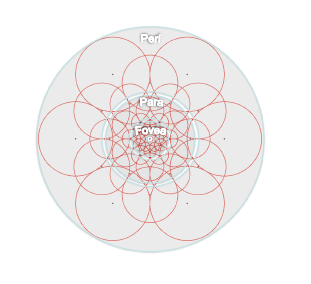
\includegraphics[width=60mm]{figures/freak_descriptor} \\
(a) The retinal pattern in the eye (b) The pattern of FREAK descriptor \\[6pt]
\end{tabular}
\caption{The FREAK feature descriptor} \label{fig:freak_descriptor}
\end{figure}


\subsection {KAZE and A-KAZE} \label{subsec:kaze_akaze}
KAZE (Japanese word meaning \emph{wind}) \cite{alcantarilla2012kaze} feature is a new 2D multi-scale feature detection and description that its algorithm rely on nonlinear scale space. Previous methods such as SIFT or SURF find features in the Gaussian scale space (particular instance of linear diffusion). However, Gaussian blurring does not respect the natural boundaries of objects and smooths in the same degree details and noise when evolving the original image through the scale space.\\
By means of nonlinear diffusion we can detect and describe features in nonlinear scale spaces keeping important image details and removing noise as long as we evolve the image in the scale space. We use variable conductance diffusion which is one of the simplest cases of nonlinear diffusion. The nonlinear scale space is build efficiently by means of Additive Operator Splitting (AOS) schemes, which are stable for any step size and are parallelizable.\\
A-KAZE (Accelerated-KAZE) \cite{alcantarilla2011fast} Features uses a novel mathematical framework called Fast Explicit Diffusion (FED) embedded in a pyramidal framework to speed-up dramatically the nonlinear scale space computation. In addition, we compute a robust Modified-Local Difference Binary (M-LDB) descriptor that exploits gradient information from the nonlinear scale space. A-KAZE obtains comparable results to KAZE in some datasets, while being several orders of magnitude faster.\\
% TODO: check the speed
Despite of moderate increase in computational time, especially compare to SURF, the AKZE feature algorithms is a forward step in performance and accuracy for both detection and description against previous state-of-the-art algorithms such as SURF, SIFT, BRISK and FREAK.
The below graphs are taken form computer-vision-talks weblog \footnote{\url{http://computer-vision-talks.com/articles/2013-03-17-porting-kaze-features-to-opencv/}} and prepared by OpenCV Comparison Tool \footnote{\url{https://github.com/BloodAxe/OpenCV-Features-Comparison}}. It compares the KAZE feature with the other well-known algorithms from several aspects of invariance such as rotation, scale and brittleness and robustness to blur. As you can see, in all cases, the result of KAZE is strongly effective and better than others. 

\begin{figure}[H]
\begin{tabular}{cc}
  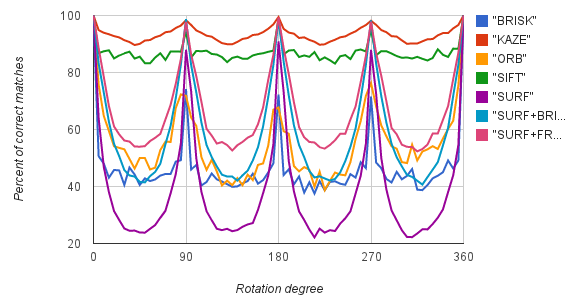
\includegraphics[width=75mm]{figures/rotation_KAZE} &  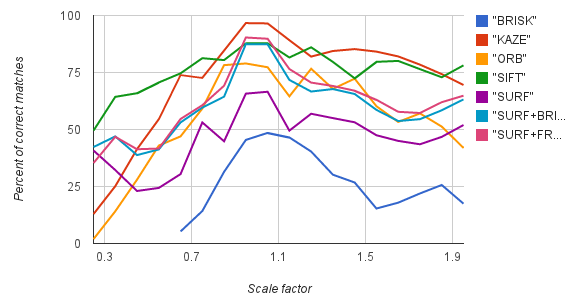
\includegraphics[width=75mm]{figures/scale_KAZE} \\
(a) Rotation Test & (b) Scale Invariance \\[6pt]
 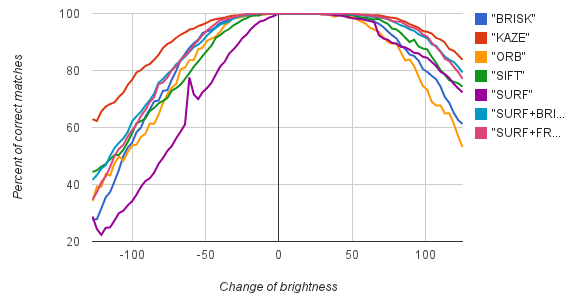
\includegraphics[width=75mm]{figures/brightness_KAZE} &  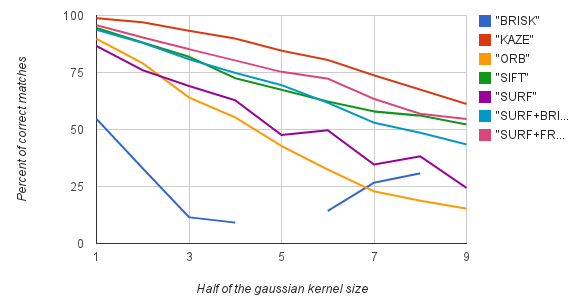
\includegraphics[width=75mm]{figures/blur_KAZE} \\
(c) Brittleness Invariance & (d) Robustness to Blur \\[6pt]
\end{tabular}
\caption{The comparison of KAZE and other well-know feature descriptions}\label{fig:compare_kaze}
\end{figure}

As we mentioned in the description of A-KAZE, it uses two new algorithms (FED and M-LDB) and consequently the computation cost for detection and description decrease dramatically. It also extends to support four different types of extracted descriptors (\detokenize{Descriptor_KAZE, Descriptor_KAZE_upright, Descriptor_MLDB and Descriptor_MLDB_upright}) depending on image properties. In the next graph, a comparison between four top binary descriptors, A-KAZE, KAZE, BRISK, FREAK, is shown. It also was prepared by computer-vision-talks weblog. All methods are tested for a variety of environments and conditions.
% $$(Descriptor_KAZE, Descriptor_KAZE_upright, Descriptor_MLDB and Descriptor_MLDB_upright)$$

\begin{figure}[H]
\begin{tabular}{cc}
  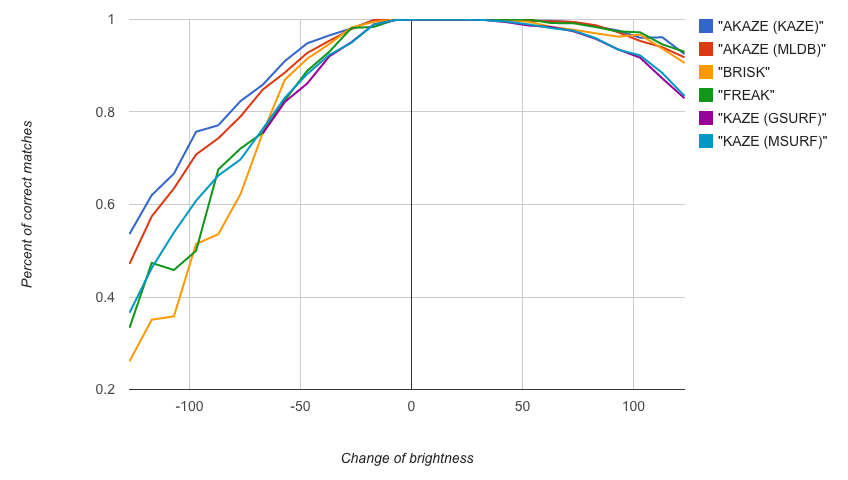
\includegraphics[width=75mm]{figures/brithness_akaze} &  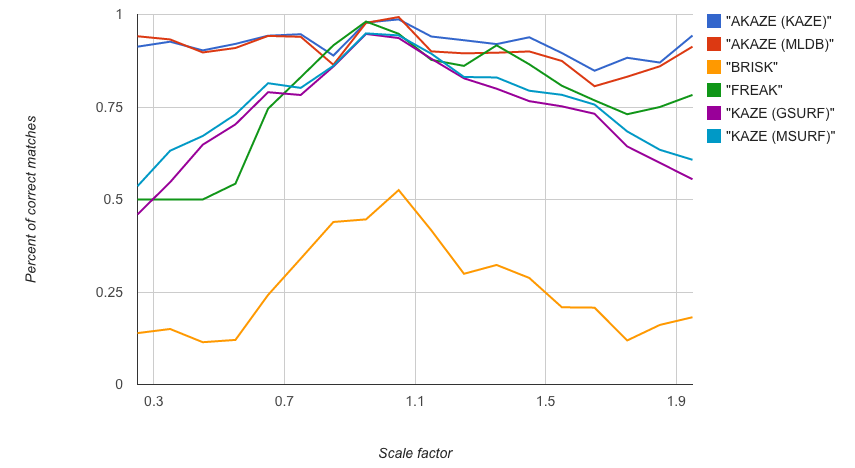
\includegraphics[width=75mm]{figures/scale_akaze} \\
(a) Brittleness Invariance & (b) Scale Invariance \\[6pt]
\multicolumn{2}{c}{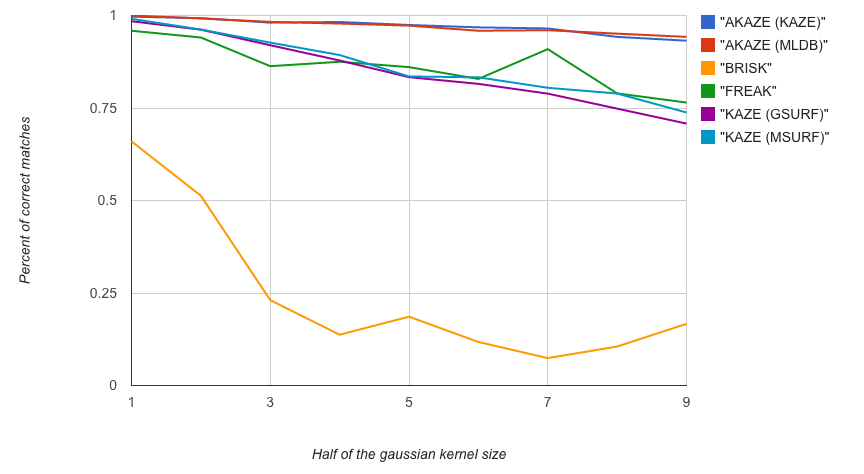
\includegraphics[width=75mm]{figures/blur_akaze} }\\
\multicolumn{2}{c}{(e) Robustness to Blur}
\end{tabular}
\caption{The comparison between KAZE and A-KAZE}\label{fig:compare_kaze_and_A-kaze}
\end{figure}

% TODO : add new test and combines with next paragraph.
Beside of the original author's implementation \footnote{\url{https://github.com/pablofdezalc/akaze}}, both KAZE and A-KAZE are ported to the new version of OpenCV 3.0  \footnote{\url{http://docs.opencv.org/trunk/modules/features2d/doc/feature_detection_and_description.html}} and boosted by OpenCL. In this master thesis, the OpenCV's A-KAZE is utilized for both feature detection and description procedures. 
% The parameters of A-KAZE optimized based of our requirement and listed as below table:

% \begin{table}[H]
%   \caption{A-KAZE value parameters in OpenCV 3.0}
%   \begin{tabular}{| c | c | c | c | c | c | c |}
%       \hline
%       descriptor type & descriptor size & descriptor channels & threshold & octaves & sublevels & diffusivity \\ \hline \hline
%       Descriptor dump & Full & 3 & 0.001 & 4 & 4 & dump \\ \hline
%   \end{tabular}
% \end{table}

In this master thesis we were looking for a best feature descriptor that should be invariant to brightness, scale, rotation and be robust to blur. Between all feature detectors and extractors that already mentioned here, the KAZE (Japanese word meaning \emph{wind}) and especially A-KAZE feature detector and extractor was selected as the best candidate. Right now it has the best result among all algorithms in this subject.

\subsection {cvAKAZEFeature} \label{subsec:cv_akaze_feature}
% TODO: master thesis reference
% TODO: Ubitrack
In Ubitrack, some basic classes that represent the feature descriptor and feature matching, were implemented by Sven Barth \cite{barth2014marker}. The basic class of that implementation is an abstract class with name FeatureBase. This class is used for dynamic casting between different kind of feature points that we have.
The next class in this hierarchy that is inherited from FeatureBase is Feature class. The Feature class that consists of a  \detokenize{boost::shared_ptr} of FeatureBase that represents the location of a feature point and a \detokenize{Math::Pose} object that is used for storing the position of the object relative to the camera. The \detokenize{Math::Pose} involves rotation and translation matrices. To cover the OpenCV feature point (implemented by OpenCV), class OpenCVFeature is extended from Feature class. It consists of a \detokenize{cv::keypoint} for storing the data of feature point and \detokenize{cv::Mat} for its feature descriptor vector (binary or float). The cvAKAZEFeature is a sub class of OpenCVFeature that is used for saving the value of AKAZE's feature point and descriptor. The \autoref{fig:cv_akaze} illustrates the hierarchy of cvAKAZEFeature.

\begin{figure}[H]
  \centering
  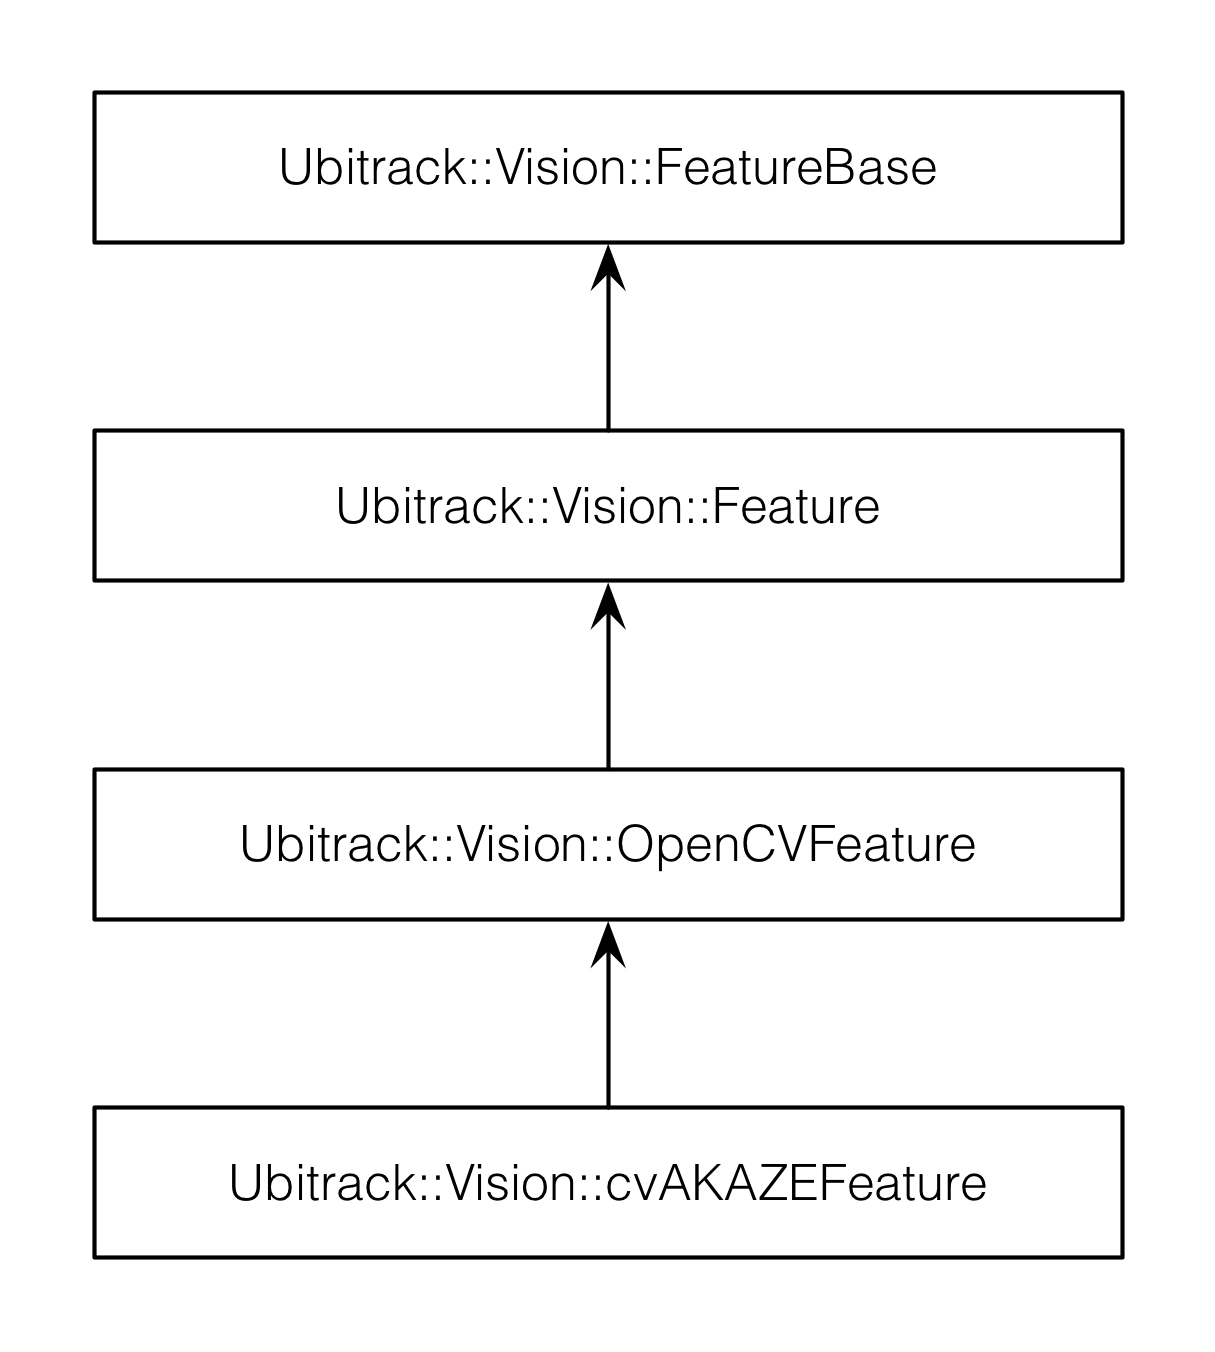
\includegraphics[width=65mm]{figures/cv_akaze}
  \caption{The hierarchy of cvAkazeFeature class in Ubitrack Framework}\label{fig:cv_akaze}
\end{figure}

In the case of implementation, The input of cvAKAZEFeature is a RGB Image and the output result is a vector of feature descriptor. \autoref{fig:cv_akaze_feature} demonstrates the data flow of our cvAKAZEFeature module.

\begin{figure}[H]
  \centering
  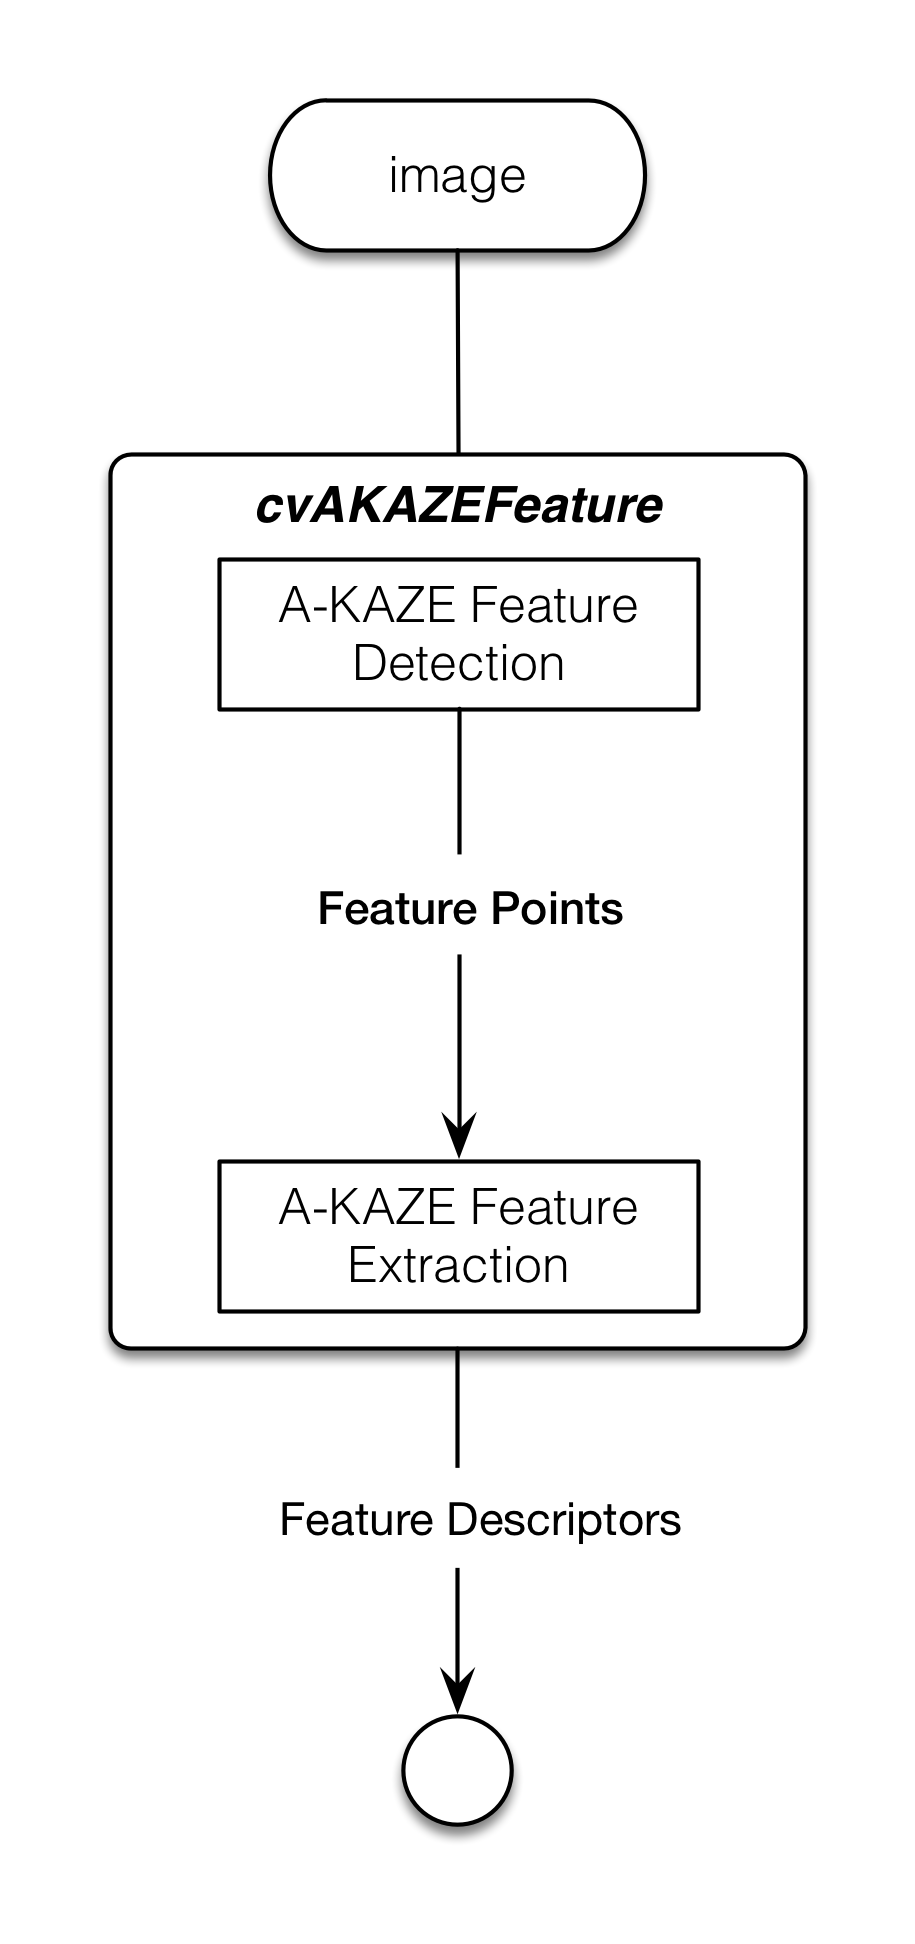
\includegraphics[width=45mm]{figures/cv_akaze_feature}
  \caption{the data flow of cvAKAZEFeature module}\label{fig:cv_akaze_feature}
\end{figure}
